\section{Performance}

The response of the LTCC to pions has been studied using experimental data containing ``good'' pion tracks.
The event selection is described below.

\subsection{Pions Selection}

First, only events with ``good'' electrons are considered. These are electrons with a cut on the ECAL sampling fraction.

To identify positive pions, events with a positive track candidates $t^+$ are considered and a cut on the the neutron missing mass $e^-t^+(n)$
is applied between 0.7 and 1.1 GeV (see \F{neutronMM}).

%To identify negative pions, events with a positive track $t^+$ are considered and a cut on the the neutron missing mass $e^-t^+(n)$
%is applied between 0.7 and 1.1 GeV (see \F{neutronMM}).


\begin{figure}
	\centering
	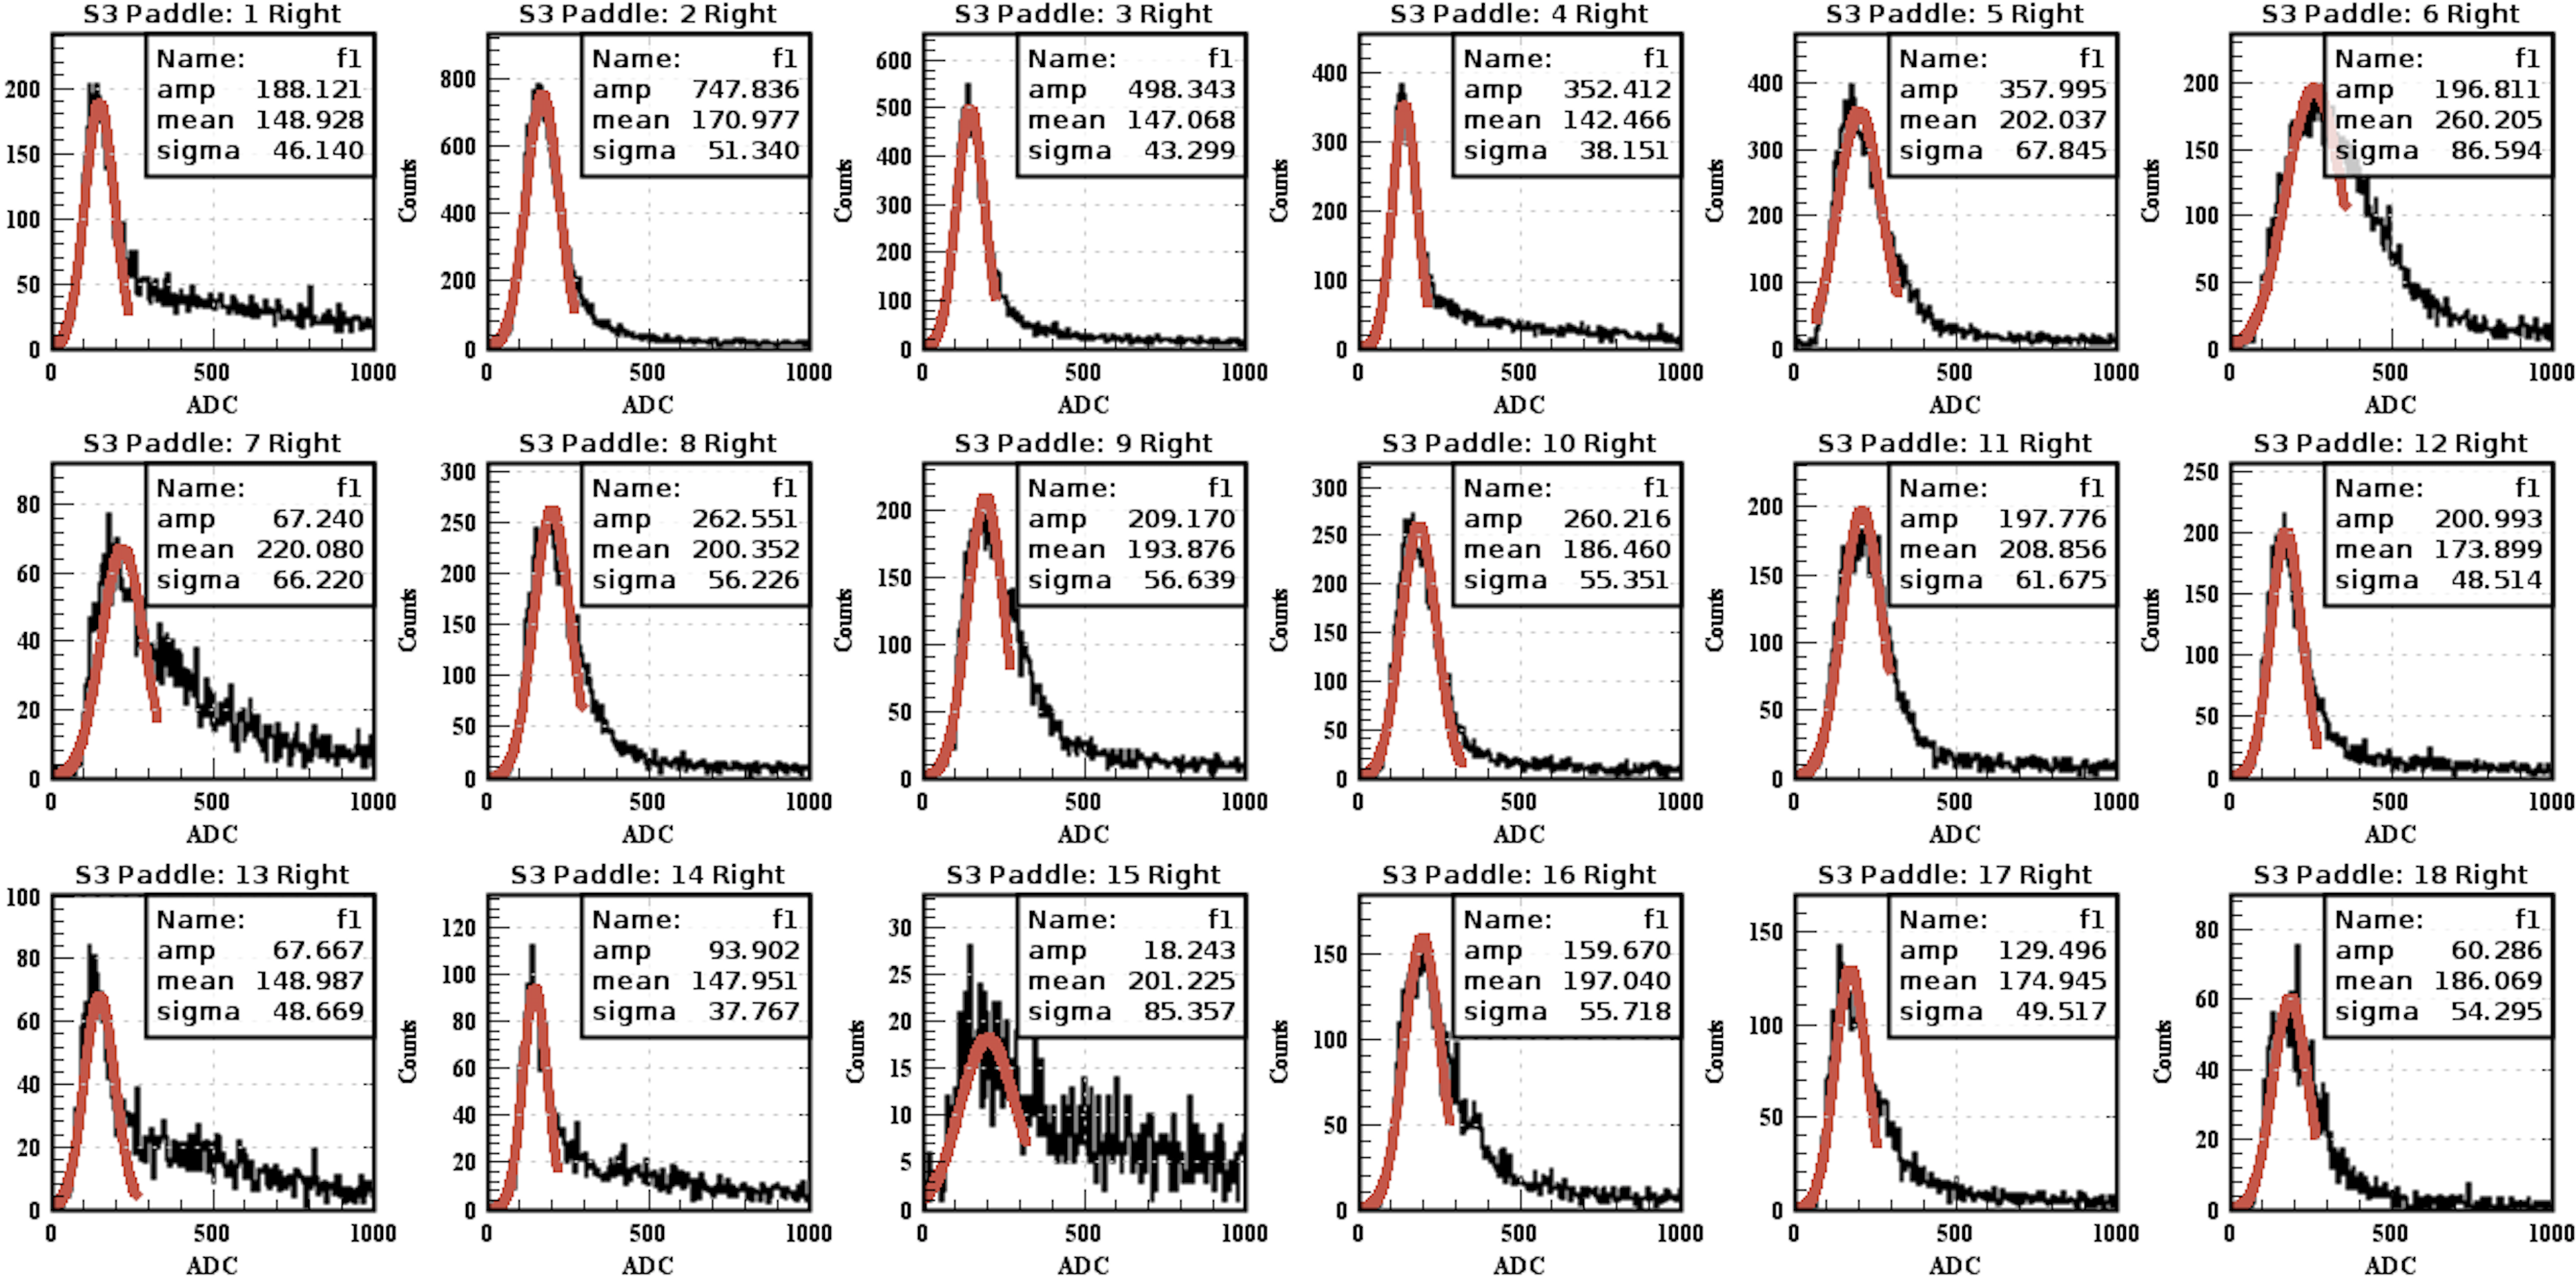
\includegraphics[width=0.98\columnwidth,keepaspectratio]{img/neutronMM.png}
	\caption{The neutron missing mass $e^-t^+(n)$.  }
	\label{fig:neutronMM}
\end{figure}






\subsection{LTCC Pions Rsponse}

2 d plots of number of photoelectrons for both positive and negative pions


\begin{figure}
	\centering
	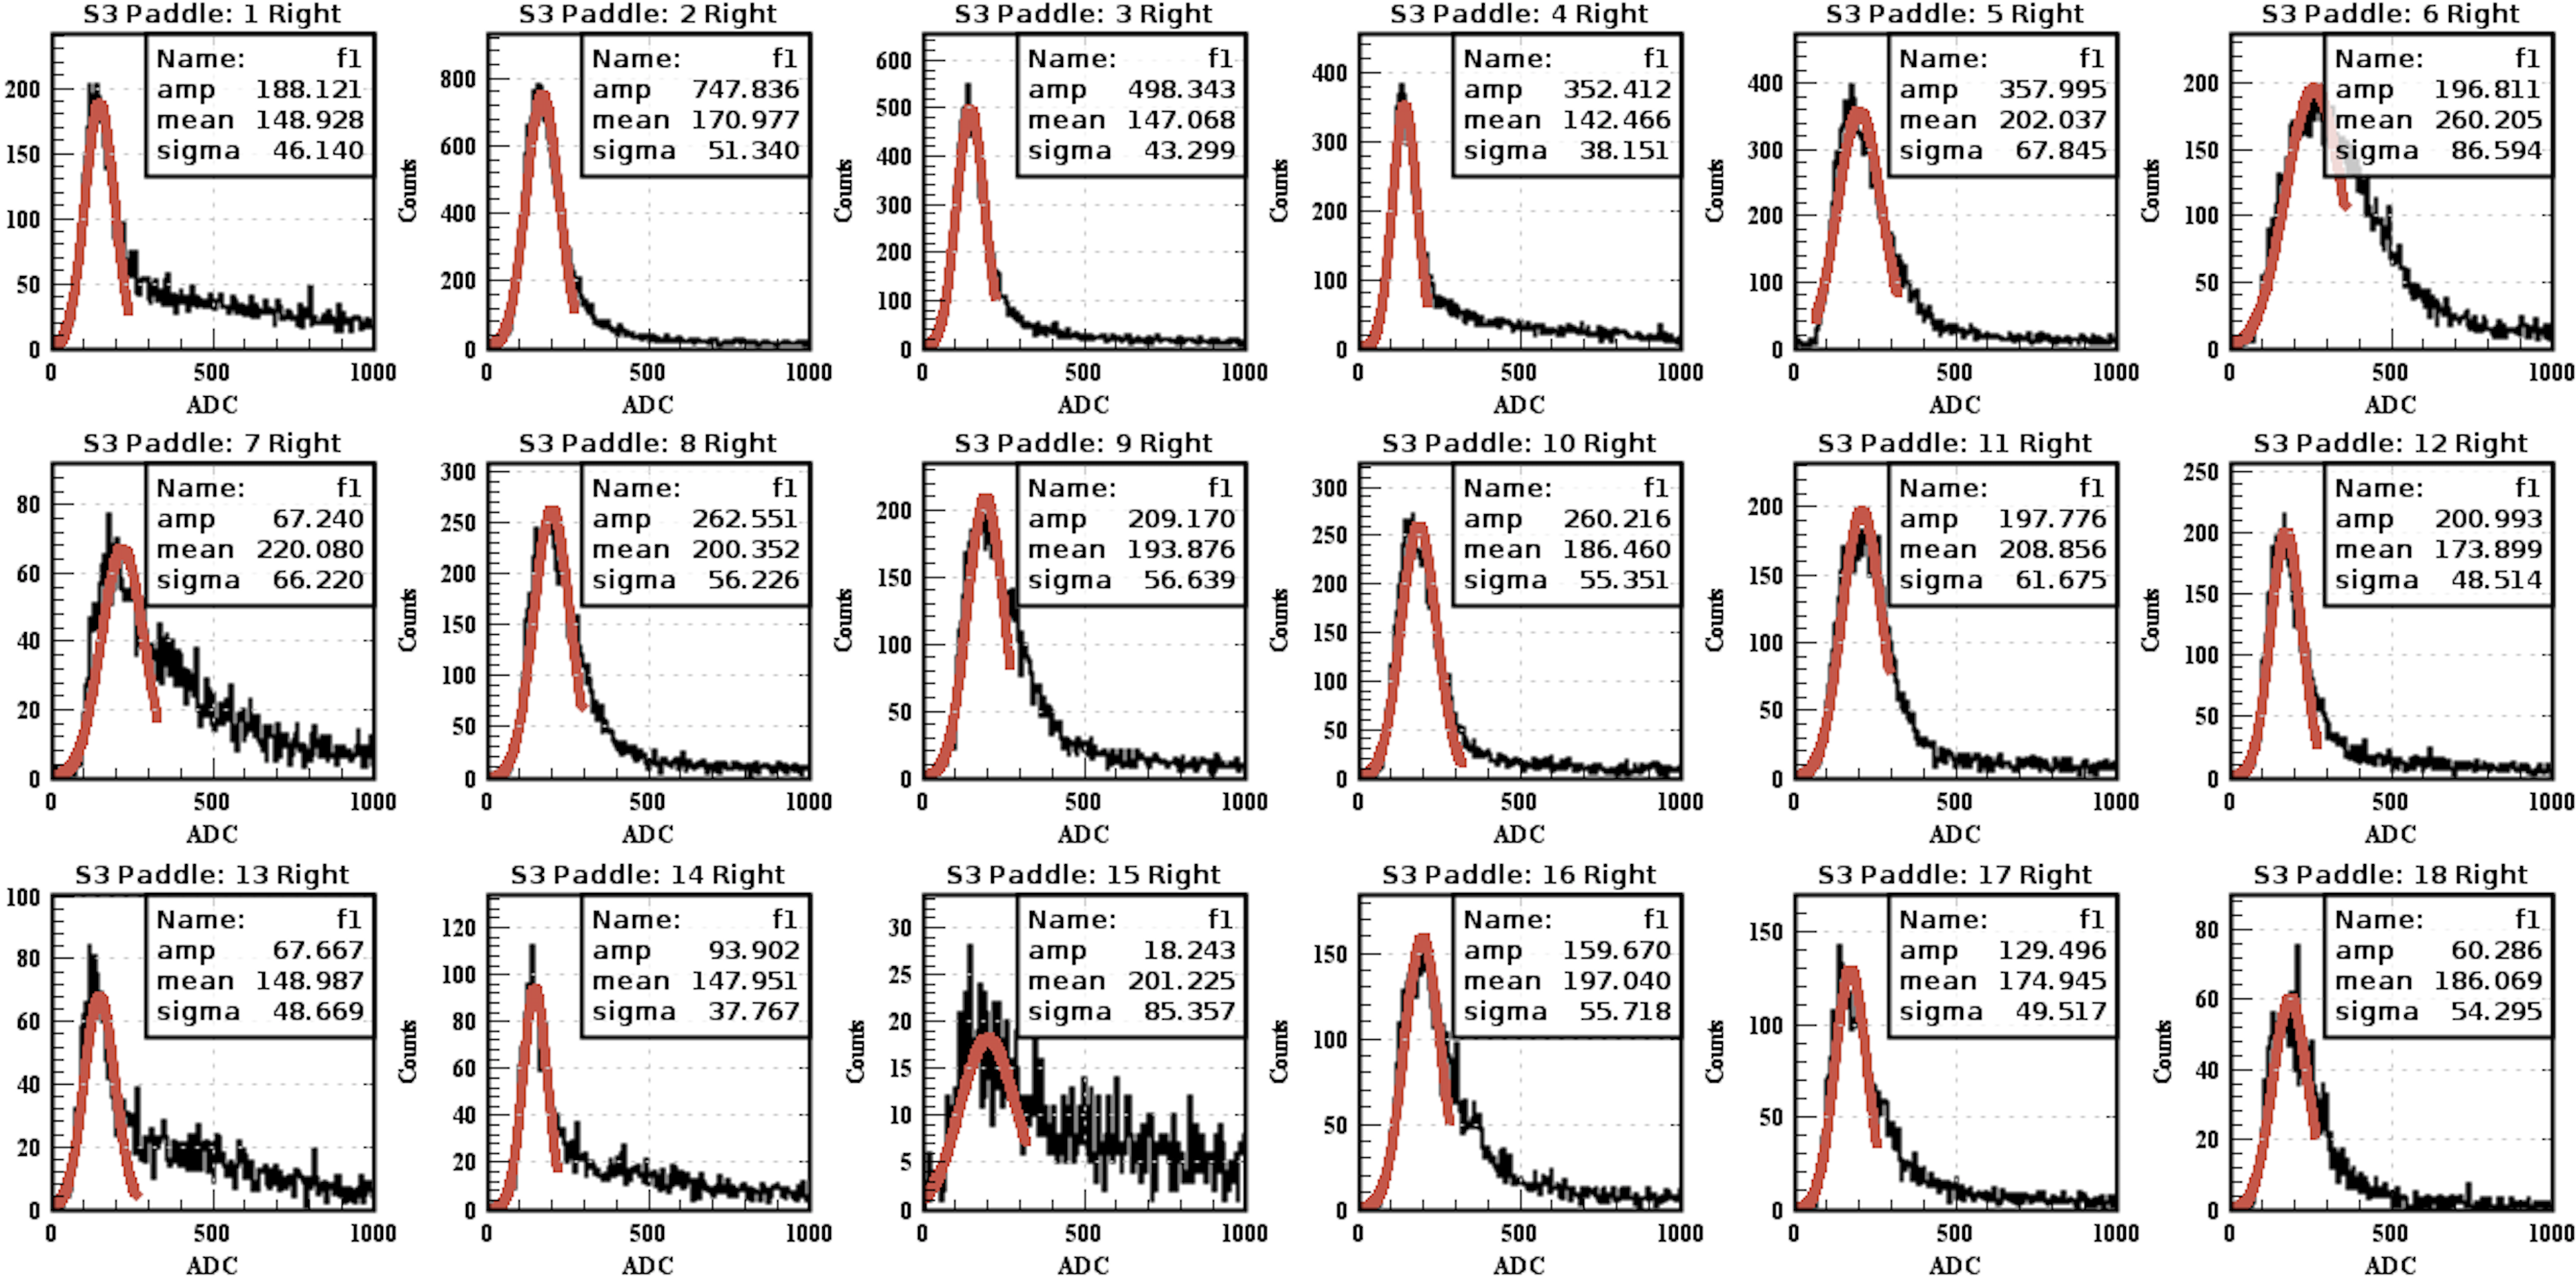
\includegraphics[width=0.98\columnwidth,keepaspectratio]{img/pipnphe.png}
	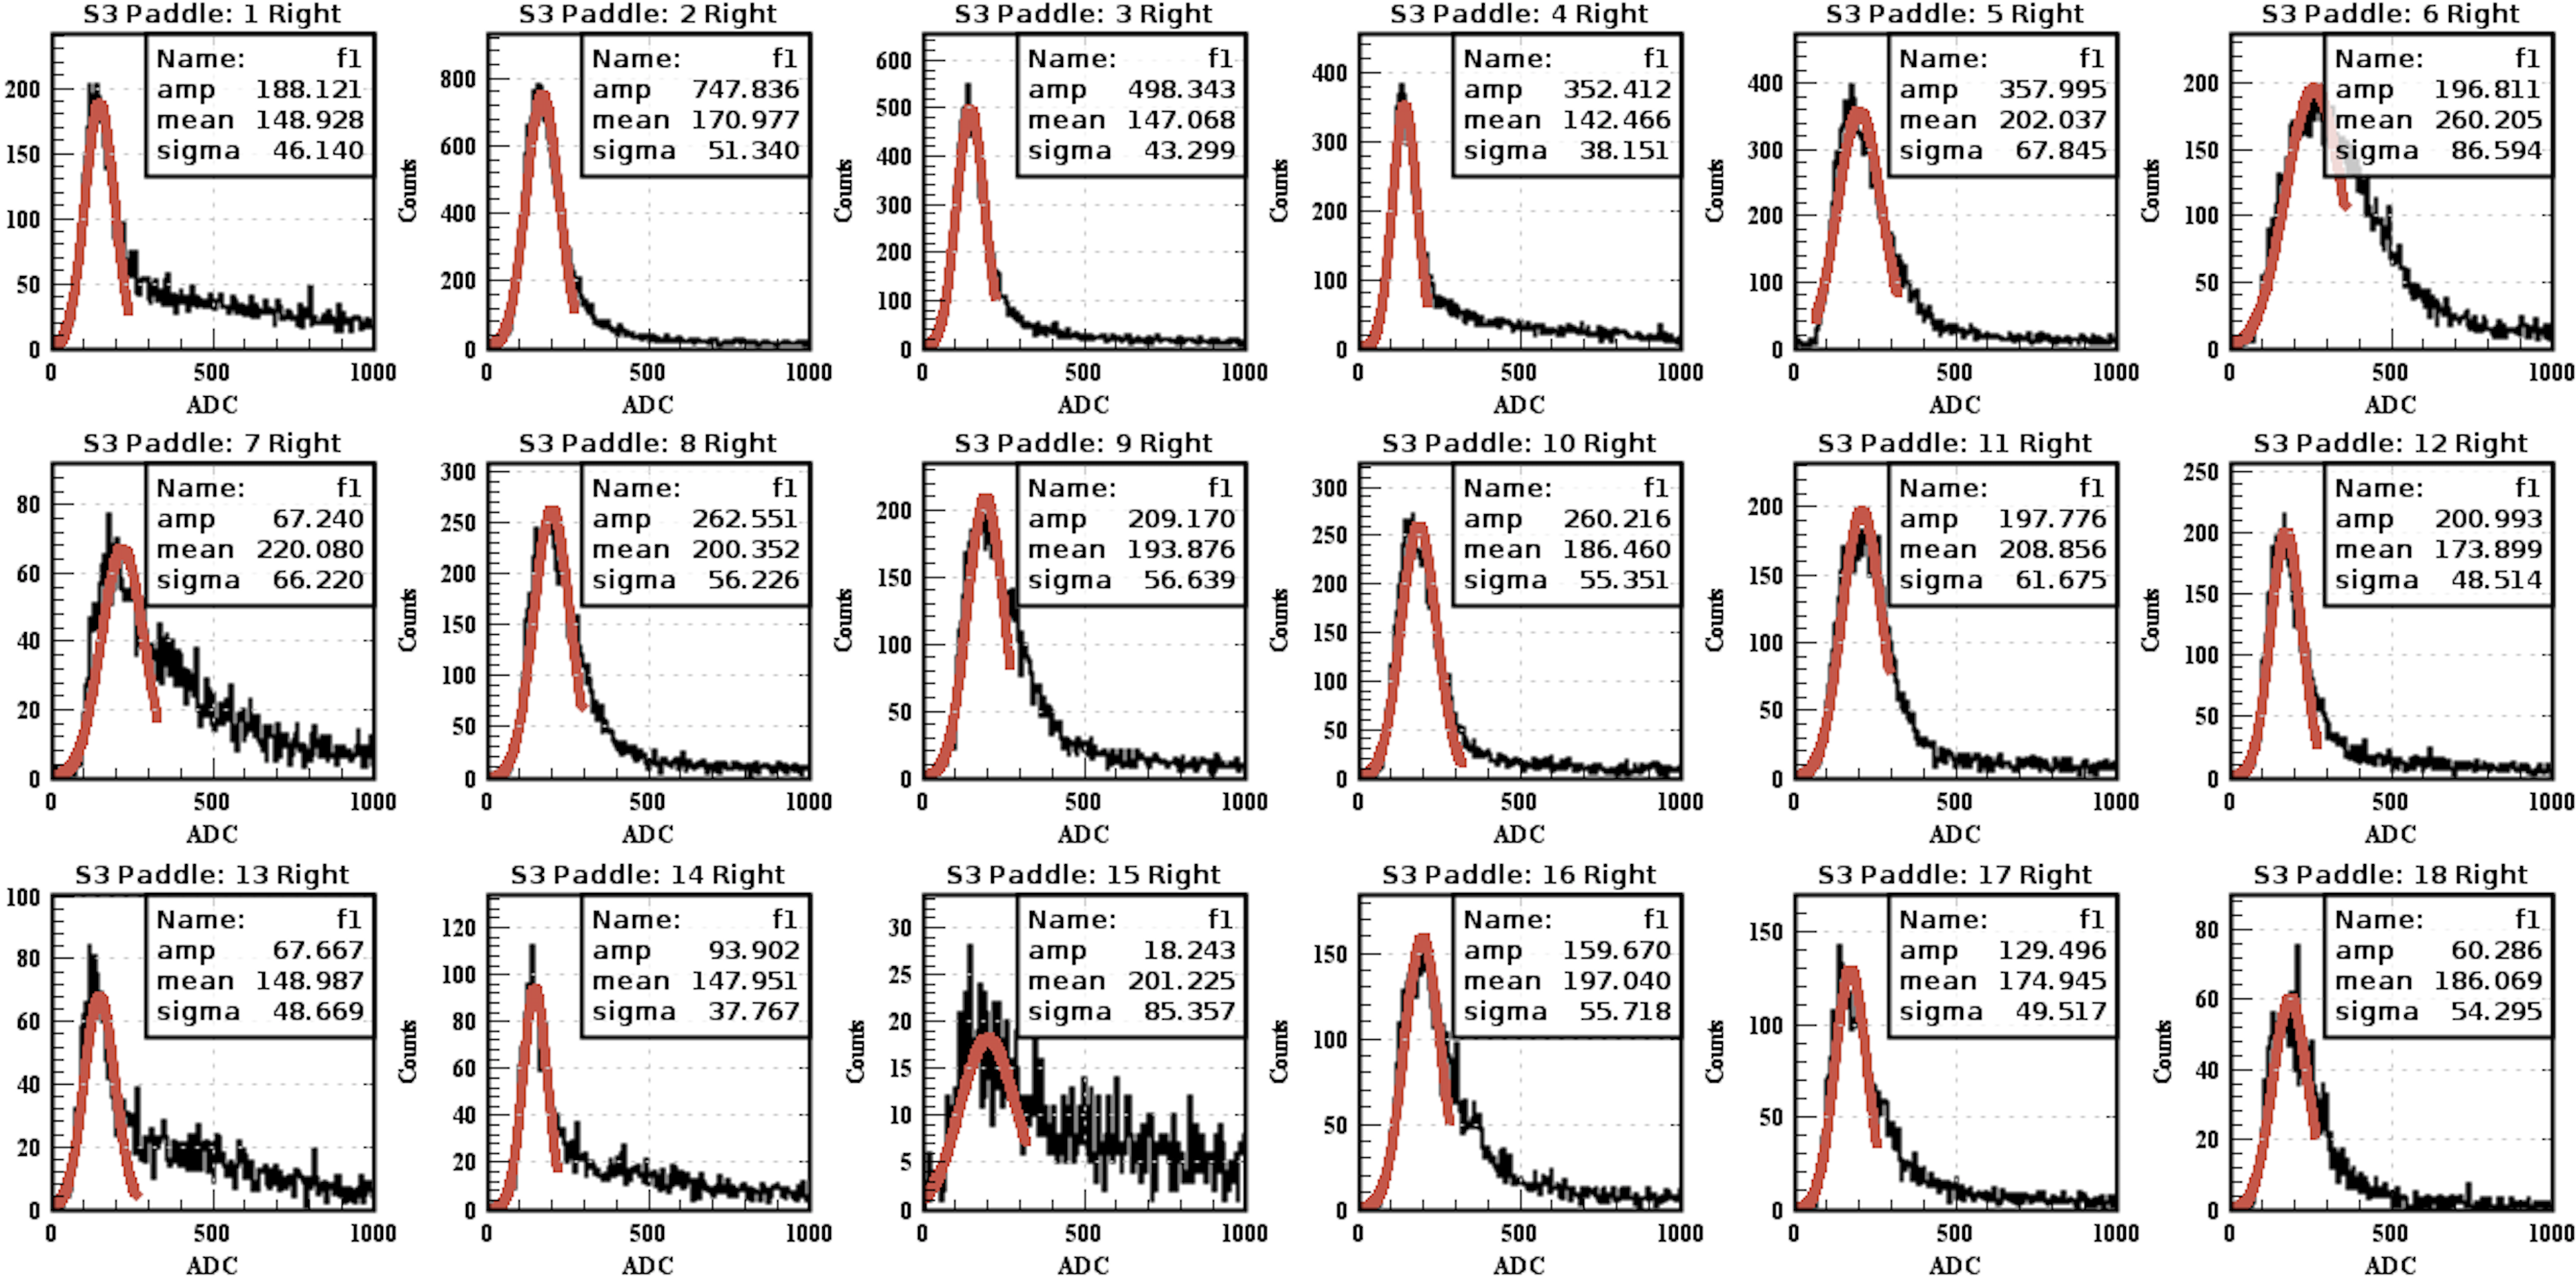
\includegraphics[width=0.98\columnwidth,keepaspectratio]{img/pimnphe.png}
	\caption{The number of photoelectrons as a function of $\theta$ and $\phi$ for 5 to 7 GeV pions. Top: positive pions. Bottom: negative pions}
	\label{fig:neutronMM}
\end{figure}



